\subsection{Stabilitet}
\label{effektforstaerker-stabilitet}

For at sikre at effektforstærkeren ikke er ustabil skal en fasemargin på mindst 45\degree~ opnås. For at kunne vurdere hvorvidt der er et problem i det nuverænde kredsløb, vel at mærke uden C2 vist på figur \ref{fig:effektkredsloeb}, simuleres kredsløbet uden AC-tilbagekobling men med DC. Måden hvorpå dette gøres i LTspice er vist i bilag \cite{effektforstaerker-openloop-simulering}%\kilde{til billede af openloop effektforstærker fra LTspice}
. Simuleringen viser at der, ved 0 dB er en fasemargin på -33\degree~. For at opnå en acceptabel fasemargin identificeres det trin som indeholder den dominerende pol for derefter at flytte polen. På figur \ref{fig:frek_openloop_ukorigeret} vises open-loop frekvenskarakteristikken for differensforstærkeren, blå, spændingsforstærkeren, rød, og hele effektforstærkeren, grøn. 


\begin{figure}[h]
\centering
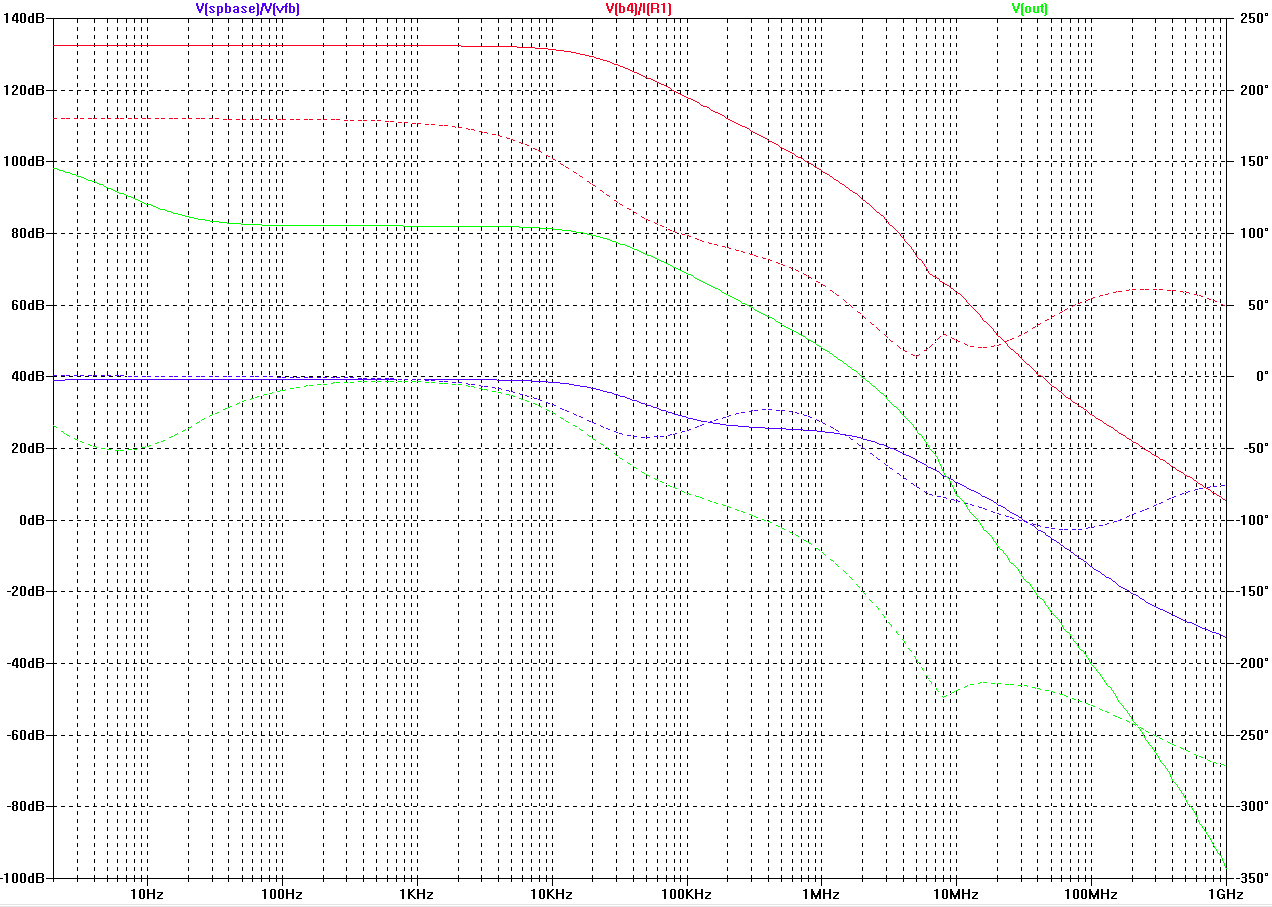
\includegraphics[width=\textwidth]{teknisk/effektforstaerker/frek_ukorrigeret_stabilitet.png}
\caption{Simuleret open-loop frekvenskarakteristik for differensforstærkeren, blå, spændingsforstærkeren, rød, og hele effektforstærkeren, grøn}
\label{fig:frek_openloop_ukorigeret}
\end{figure}

Her kan det ses at den dominerende pol skyldes spændingsforstærkeren. Det vurderes at denne knækfrekvens skyldes parasitkapaciteten, $C_\mu$, i transistor Q6. Ved at ændre værdien på $C_\mu$ kan polen flyttes. For at verificere at knækfrekvens som ses på simuleringen bliver lavet af $C_\mu$ beregnes den med tidskonstantmetoden vist i formel \ref{eq:knaekberegning_openloop} \cite{tidskonstantmetoden} %\kilde{mm11 notes i bilag}
hvor $C_1$ og $C_2$ er henholdsvis den millertransformerede $C_\mu$ på indgang og udgangen.

\begin{equation}
f_p=\frac{1}{(r_\pi \cdot (C_\pi + C_1) + R_L \cdot C_2) \cdot 2 \cdot \pi}
\label{eq:knaekberegning_openloop}
\end{equation}

$C_1$ og $C_2$ er givet ved formel \ref{eq:miller1} og \ref{eq:miller2} hvor K er råforstærkningen i spændingsforstærkeren.

\begin{equation}
C_1=C_\mu \cdot \left( 1-K \right)
\label{eq:miller1}
\end{equation}
\begin{equation}
C_2=C_\mu \cdot \left( 1-\frac{1}{K} \right)
\label{eq:miller2}
\end{equation}

For at være sikker på at beregningerne kan sammenlignes med simuleringerne beregnes der ud fra samme værdier for $C_\mu$, K, $C_\pi$ som simuleringsprogrammet benytter. Værdierne aflæses til følgende: 

\[ C_\mu=1,6~\mathrm{pF} \]
\[ C_\pi=153~\mathrm{pF} \]
\[ r_\pi=2,97~\mathrm{k}\ohm \]
\[ K=63 \mathrm{dB} \approx -1412~\mathrm{gange}\]

Dermed kan knækfrekvensen, $f_p$ beregnes i formel \ref{eq:polverifikation}, hvor $R_L$ er spændingsforstærkerens belastning, som er beregnet i afsnit \ref{effekt_spaendingsforstaerker}.
\begin{equation}
f_p=\frac{1}{(r_\pi \cdot (C_\pi + C_\mu \cdot \left( 1-K \right)) + R_L \cdot C_\mu \cdot \left( 1-\frac{1}{K} \right)) \cdot 2 \cdot \pi}=22~\mathrm{kHz}
\label{eq:polverifikation}
\end{equation}

Knækfrekvensen er på simuleringen aflæst til 20 kHz hvormed det vurderes at beregningen på 22 kHz er tæt nok på til at blive anset som værende korrekt. 
Da den dominerende pol nu er identificeret vides nu at capaciteten $C_\mu$ skal ændres i størrelse for at flytte knækfrekvensen, for dermed at opnå en højere fasemargin. Ved at resonere over simuleringsresultaterne er det bestemt at knækfrekvensen skal flyttes til 200 Hz for at opnå tilstrækkeligt fasemargin. I formel \ref{knaekberegning} beregnes capaciteten som $C_\mu$ skal hæves med ved at isolere $C6$. I formlen er $f_\mathrm{p1}$ sat til 200 Hz. 

\begin{equation}
f_\mathrm{p1}=\frac{1}{(r_\pi \cdot (C_\pi + (C_\mu + C6) \cdot \left( 1-K \right)) + R_L \cdot (C_\mu + C6) \cdot \left( 1-\frac{1}{K} \right)) \cdot 2 \cdot \pi} \Rightarrow C6=144~\mathrm{pF}
\label{knaekberegning}
\end{equation}

Ved at indsætte 144 pF parallel med $C_\mu$ i simuleringen opnås en fasemargin på 57\degree, som vist på figur \ref{openloop_efter_korrektion}.

\begin{figure}[h]
\centering
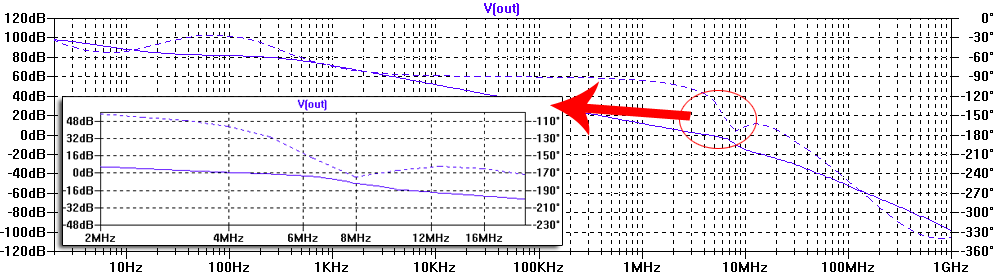
\includegraphics[width=\textwidth]{teknisk/effektforstaerker/stabilitet-medc-graf.png}
\caption{Simuleret open-loop frekvenskarakteristik for differensforstærkeren hvor polen er flyttet}
\label{openloop_efter_korrektion}
\end{figure}